\documentclass[a4paper, 12pt]{article}%тип документа

%отступы
\usepackage[left=1cm,right=1cm,top=1cm,bottom=3cm,bindingoffset=0cm]{geometry}

%Русский язык
\usepackage[T2A]{fontenc} %кодировка
\usepackage[utf8]{inputenc} %кодировка исходного кода
\usepackage[english,russian]{babel} %локализация и переносы

%Вставка картинок
\usepackage{graphicx}
\graphicspath{{pictures/}}
\DeclareGraphicsExtensions{.pdf,.png,.jpg}

%Графики
\usepackage{pgfplots}
\pgfplotsset{compat=1.9}

%Математика
\usepackage{amsmath, amsfonts, amssymb, amsthm, mathtools}

%Заголовок
\author{Валеев Рауф Раушанович \\
группа 825}
\title{\textbf{Работа 1.2.3 \\
Определение момента инерции твердых тел с помощью трифилярного подвеса}}

\begin{document}
\maketitle
\newpage
\textbf{Цель работы:} измерение момента инерции ряда тел и сравнение результатов с расчетами по теоретическим формулам; проверка аддитивности моментов инерции и справедливости формулы Гюйгенса-Штейнера.

\textbf{В работе используются:} трифилярный подвес, секундомер, счетчик числа колебаний, набор тел, момент инерции которых надлежит измерить (диск, стержень, полый цилиндр и другие).
\center{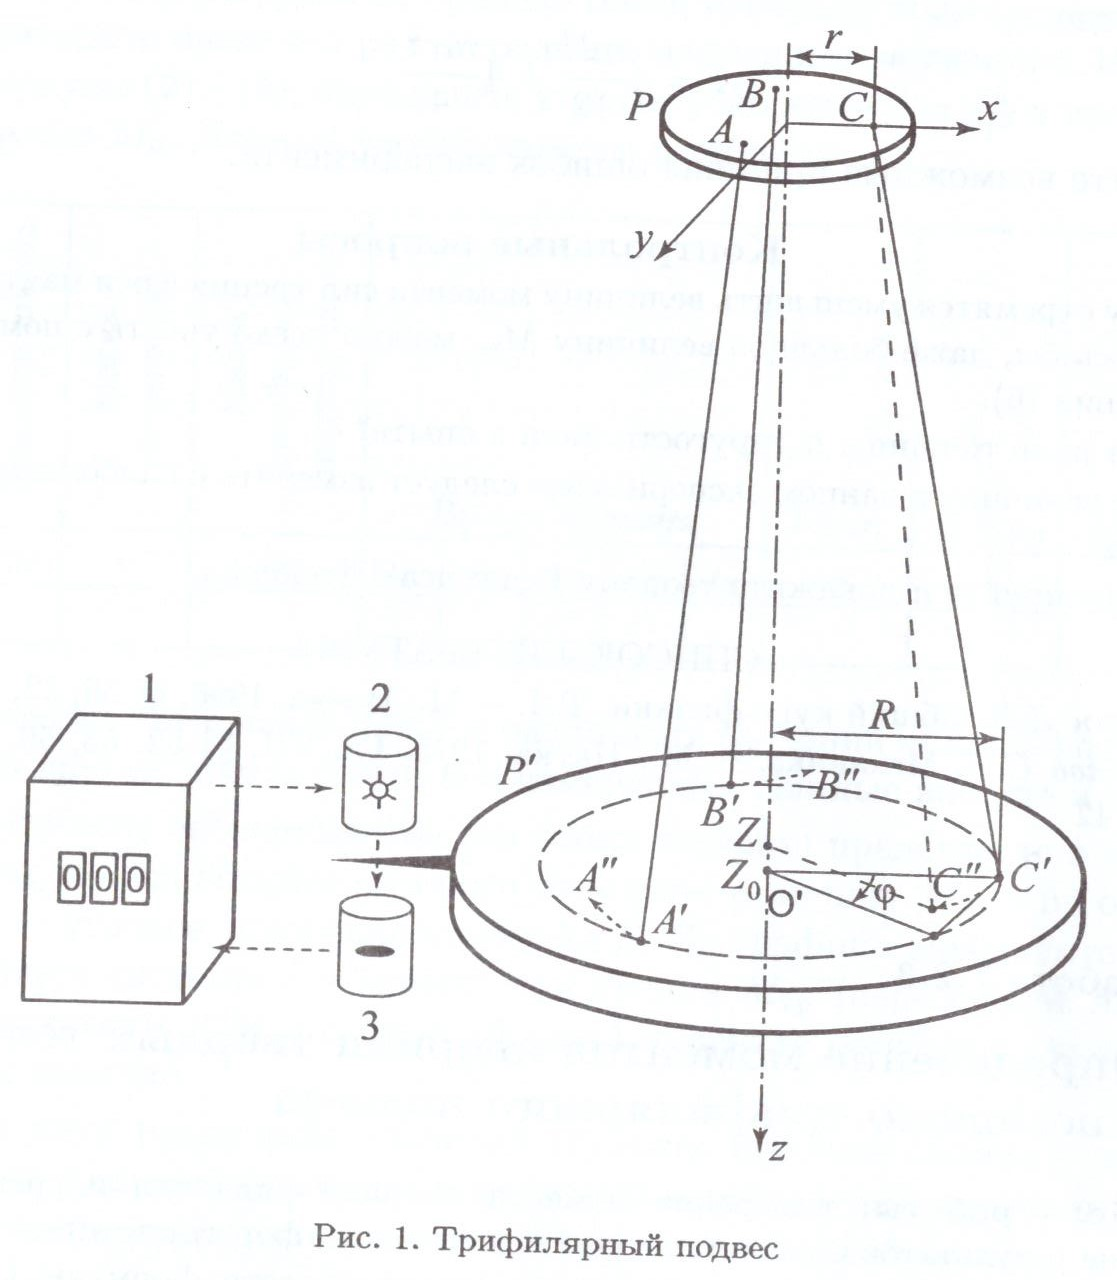
\includegraphics{123_1.jpg}}
\begin{enumerate}
\item Проверяем пригодность установки (рис. 1) для возбуждения крутильных колебаний. 
\item Проверяем, что время изменения периода крутильных колебаний в 2-3 раза много больше периода колебаний. Проверяем для ненагруженной платформы. 
\item Находим оптимальную амплитуду, то есть такую, чтобы период не зависел от амплитуды колебаний, так как запускали по кнопке, то это примерно половина от максимальной амплитуды, которую мы можем сделать. 
\item Измеряем параметры $z_0 = (2,14 \pm 0,001)$ м, $R = (0,1145 \pm 0,0005)$ м, $r = (0,0305 \pm 0,0003)$ м. По ним вычисляем константу установки $k = (4,14 \pm 0,04 ) \cdot 10 ^ {-4}$ по формуле 
\[ k = \dfrac{gRr}{4 \pi^2 z_0} \]
\[ \sigma_k = k  \sqrt{\left( \dfrac{\sigma_R}{R}\right)^2 + \left( \dfrac{\sigma_r}{r}\right)^2 + \left( \dfrac{\sigma_{z_0}}{z_0}\right)^2}\]
\item Так же нам понадобятся массы всех представленных грузов: 
\[m_{platform} = (0,9347 \pm 0,0003) kg \] \\
\[  m_{ring} = (0,7479 \pm 0,0003) kg \] \\ 
\[m_{disk} = (0,5847 \pm 0,0003) kg \] \\ 
\[ m_{beam} = (	1,2728 \pm 0,0003) kg\]
\item Измеряем периоды колебаний ненагруженной платформы и платформы со каждым грузом по отдельности и с диском и кольцом (табл. 1)
\item Определяем моменты инерции каждого груза по формуле 
\[I = kmT^2\]
\[ \sigma_I = I \sqrt{\left( \dfrac{\sigma_k}{k} \right)^2 + \left( \dfrac{\sigma_m}{m}\right)^2 + 2 \left( \dfrac{\sigma_T}{T}\right)^2} \]
\item Определяем $I$ ненагруженной платформы (табл. 2).
\item Определяем момент инерции двух тел из набора сначала порознь, потом вместе (табл. 2). Проверяем аддитивность момента инерции, т.е. что $I_{together} = I_1 + I_2$. То есть $0,01428 = 0,0121
+ 0,0096 - 0,0074$ и действительно равно с погрешностью в $1 \%$.
\item Помещаем на платформу диск, разрезанный по диаметру. Постепенно его раздвигая так, чтобы центр масс оставался на оси вращения снимаем зависимость $I (h)$ (табл. 3)
\item Строим график зависимости $I(h^2)$ и определяем по нему массу и момент инерции диска.
\item Исходя из графика масса равна 1,35 кг, что равно реальной массе с точностью до $1 \%$. Так же Нулевой импульс сходится с таблицей.
\item Измеряем все теоретические значения моментов инерции грузов по формулам
\[I_{disk} = \dfrac{mR^2}{2} \]
\[I_{ring} = mR^2 \]
\[I_{platform} = \dfrac{mR^2}{2} \]
\[I_{stick} = \dfrac{mL^2}{12} \]
\end{enumerate}
\center{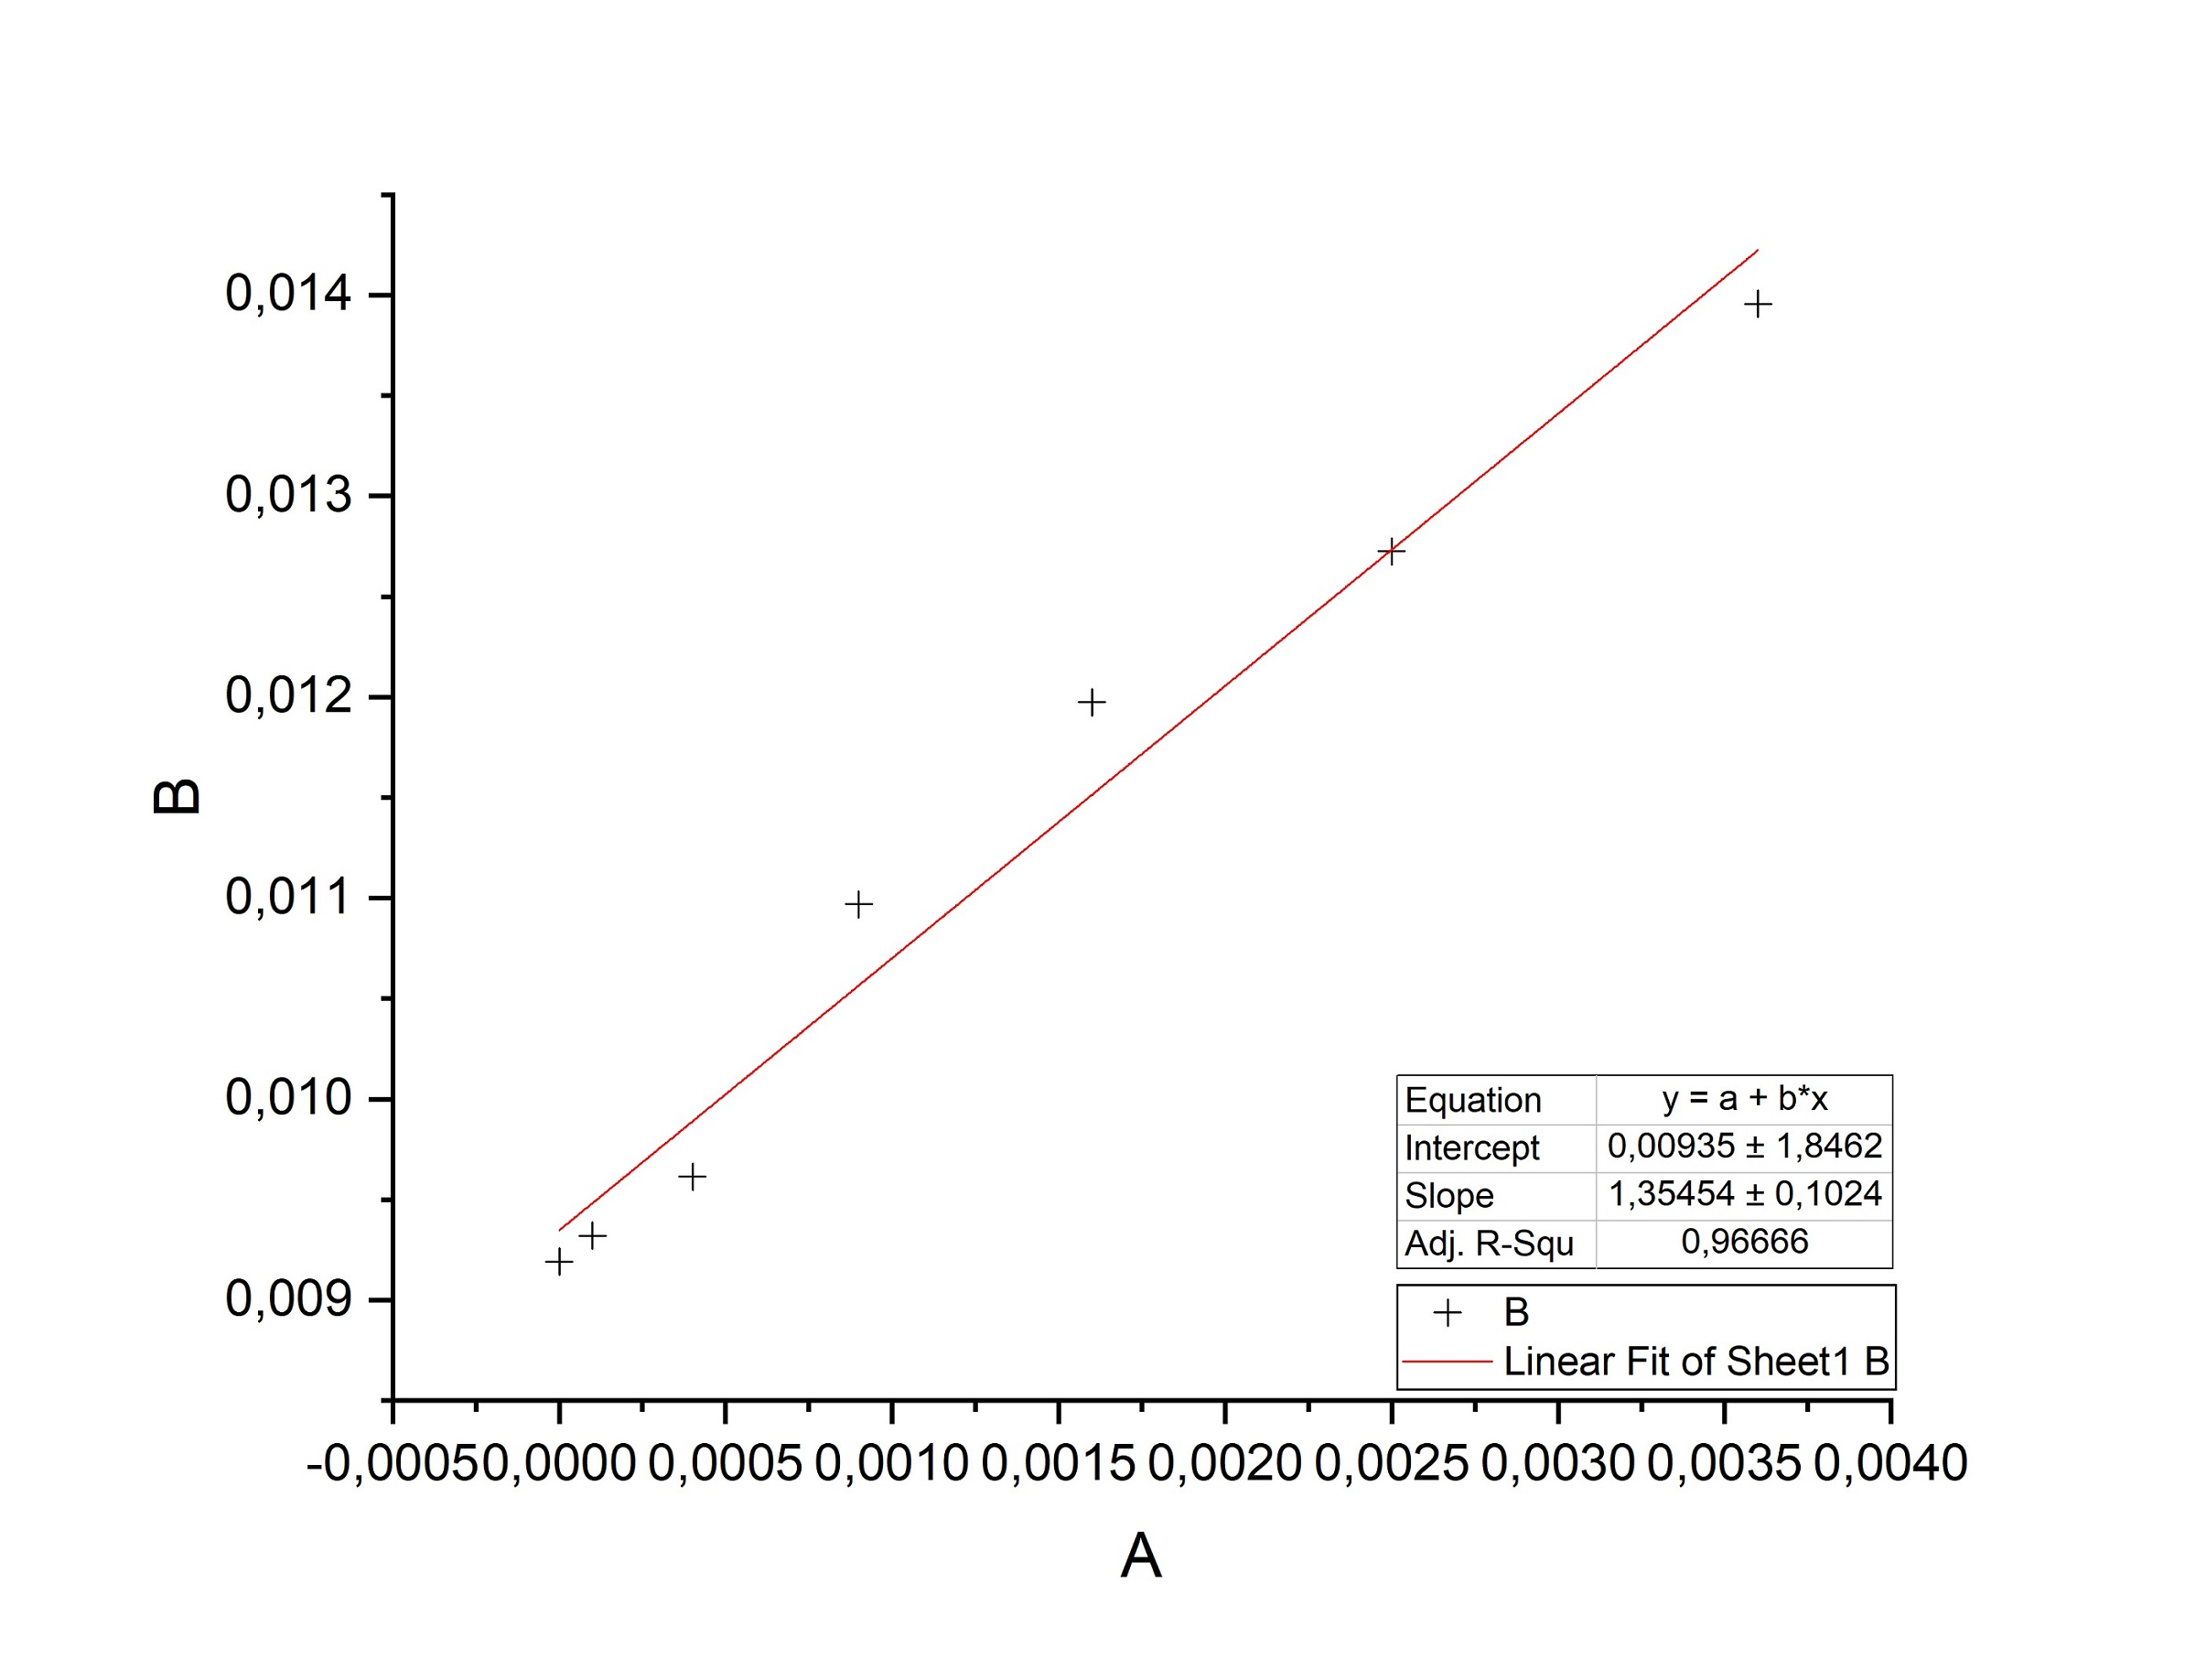
\includegraphics{123_2.jpg}}
\newpage
\center{
\begin{table}
\center{
\begin{tabular}{|c|c|c|c|c|c||c|c|}
\hline
Тело&\multicolumn{5}{|c||}{$T$, с}&$T_{sr}$, с&$\sigma_{T_{sr}}$, с\\
\hline
Платформа&4,38&4,38&4,38&4,38&4,38&4,38&0,02\\
\hline
Платформа с кольцом&4,16&4,16&4,17&4,16&4,16&4,16&0,02\\
\hline
Платформа с диском&3,91&3,91&3,91&3,91&3,91&3,91&0,02\\
\hline
Платформа с бруском&3,68&3,67&3,67&3,68&3,67&3,67&0,02\\
\hline
Платформа с диском и кольцом&3,90&3,90&3,90&3,90&3,90&3,90&0,02\\
\hline
\end{tabular}
}
\caption{$T$}
\center{
\begin{tabular}{|c|c|c|c|c|}
\hline
Тело&$I_{pract}$, $\text{кг}\cdot \text{м}^2$&$I_{teor}$, $\text{кг}\cdot \text{м}^2$&$\sigma_I$, $\text{кг}\cdot \text{м}^2$&$\varepsilon, \%$\\
\hline
Платформа&0,00744&0,00731&0,00009&2\\
\hline
Платформа с кольцом&0,0121&0,0120&0,0001&1\\
\hline
Платформа с диском&0,0096&0,0094&0,0001&2\\
\hline
Платформа с бруском&0,0123&0,0124&0,0002&1\\
\hline
Платформа с диском и кольцом&0,0143&0,0143&0,0002&0\\
\hline
\end{tabular}
}
\caption{$I$}
\begin{tabular}{|c|c|}
\hline
$T$, c&$h$, м \\
\hline
3,1258&0\\
\hline
3,1476&0,01\\
\hline
3,1968&0,02\\
\hline
3,4148&0,03\\
\hline
3,5679&0,04\\
\hline
3,6781&0,05\\
\hline
3,8518&0,06\\
\hline
\end{tabular}
\caption{$I(h)$}
\end{table}
}
\end{document}